\documentclass[aspectratio=169]{beamer}
\usepackage[utf8]{inputenc}

\usetheme{default}
\usecolortheme{seahorse}
\setbeamertemplate{navigation symbols}{}

\AtBeginSection[]
{
    \begin{frame}
        \frametitle{Table of Contents}
        \tableofcontents[currentsection]
    \end{frame}
}

\setbeamertemplate{section in toc}[sections numbered]
\setbeamertemplate{subsection in toc}[subsections numbered]

\title{What is Computing?}
\subtitle{Scientific Computing}
\author{Stefan Abi-Karam}
\date{Summer 2023}


\begin{document}

\begin{frame}
    \titlepage
\end{frame}

\begin{frame}{Table of Contents}
    \tableofcontents
\end{frame}

\section{Computers}

\begin{frame}{What is a Computer?}

    \begin{columns}
        \begin{column}{0.5\textwidth}
            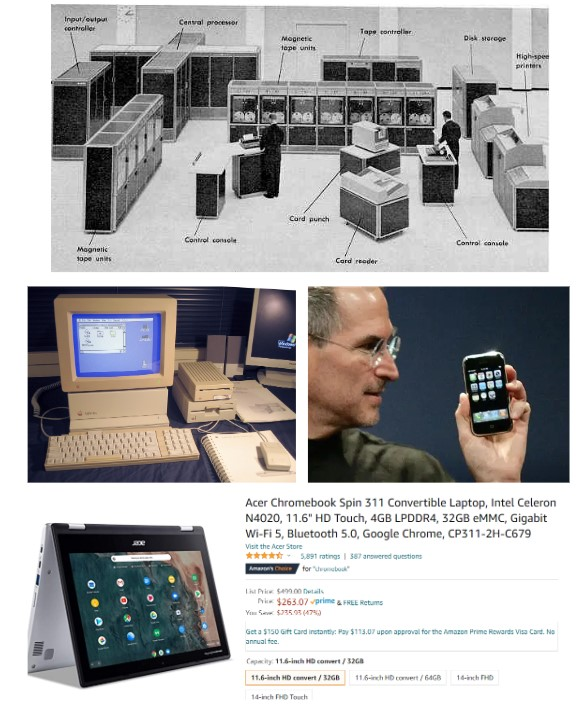
\includegraphics[width=0.8\textwidth]{imgs/vis_0.jpg}
        \end{column}
        \begin{column}{0.5\textwidth}
            A "computer" is anything that executes a set of defined instructions.

            \vspace{\baselineskip}

            \begin{itemize}
                \item We will mainly talk about computers that use electrical circuits.
                \item We can assume instructions are executed one at a time in order.
                \item In the common sense of the word, we will be talking about computers like your laptop or desktop computer (or also your phone).
            \end{itemize}
        \end{column}
    \end{columns}
\end{frame}


\begin{frame}{Operating Systems}

    Most computers we interact with have a special set of instructions call an operating system that manage a lot of the tedious task of running the computer.

    % itemize
    \begin{itemize}
        \item Manages your internet connection
        \item Manages your screen display
        \item Manages your files and storage
    \end{itemize}

    Operating systems also provide an easy way to run our own instructions to do cool stuff along with other features.

    \begin{itemize}
        \item I can run software other people wrote, like a web browser or games.
        \item I can write my own code to run on the computer to do my research stuff.
    \end{itemize}

\end{frame}

\begin{frame}{Operating Systems}

    \begin{columns}
        \begin{column}{0.5\textwidth}
            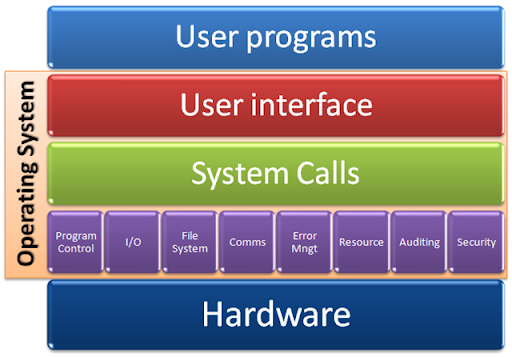
\includegraphics[width=\textwidth]{imgs/vis_1.jpg}
        \end{column}
        \begin{column}{0.5\textwidth}
            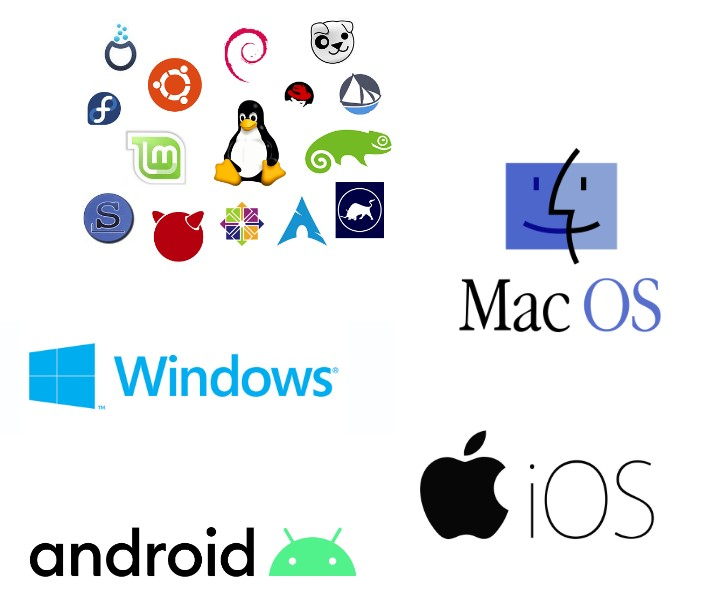
\includegraphics[width=\textwidth]{imgs/vis_2.jpg}
        \end{column}
    \end{columns}

\end{frame}

\section{Computer Hardware}

\begin{frame}{Lowest Level of a Computer}
    In the lowest level of hardware, there are several components:

    \begin{itemize}
        \item \textbf{Clock}: Keep a constant time, one tick every $x$ seconds
        \item \textbf{Registers}: Where data is stored while working with it
        \item \textbf{Arithmetic Logic Unit (ALU)}: Does the actual computations
              \begin{itemize}
                  \item Add / subtract two numbers, compare two numbers, execute logic functions (\texttt{AND}, \texttt{OR}, \texttt{INVERSE}, \texttt{XOR})
                  \item Modern computers have cool features built-in like multiply, divide, multiply-add, decimal math, etc...
              \end{itemize}
        \item \textbf{Control Logic}: Tells the computer what to do next
              \begin{itemize}
                  \item Keeps track of current instruction and next instruction
                  \item Can jump to different instructions and save current location to jump back to later
              \end{itemize}
        \item \textbf{Memory}: Where data is stored while it's waiting to be worked on
              \begin{itemize}
                  \item Temporary - gets erased when you turn off the computer
              \end{itemize}
        \item \textbf{Storage (Optional)}: Where data is stored in the long-term
              \begin{itemize}
                  \item Permanent - doesn't get erased when you turn off the computer
              \end{itemize}
    \end{itemize}

\end{frame}

\begin{frame}{Lowest Level of a Computer}
    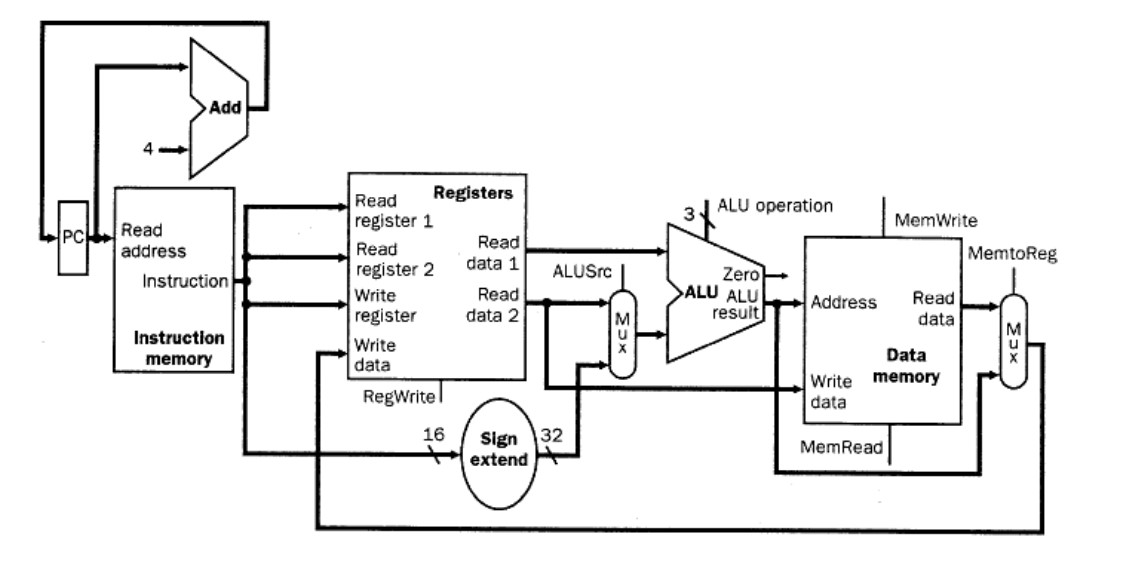
\includegraphics[width=\textwidth]{imgs/vis_3.jpg}
\end{frame}

\begin{frame}{Lowest Level of a Computer}
    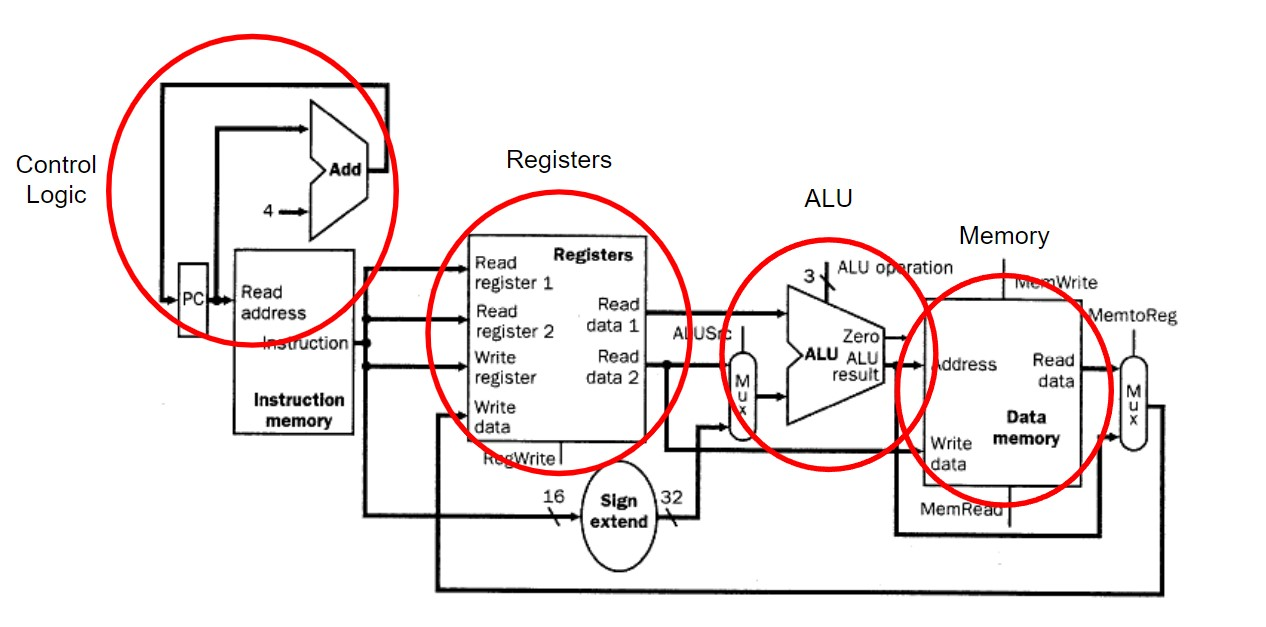
\includegraphics[width=\textwidth]{imgs/vis_4.jpg}
\end{frame}

\begin{frame}{Lowest Level of a Computer}

    \begin{columns}
        \begin{column}{0.5\textwidth}
            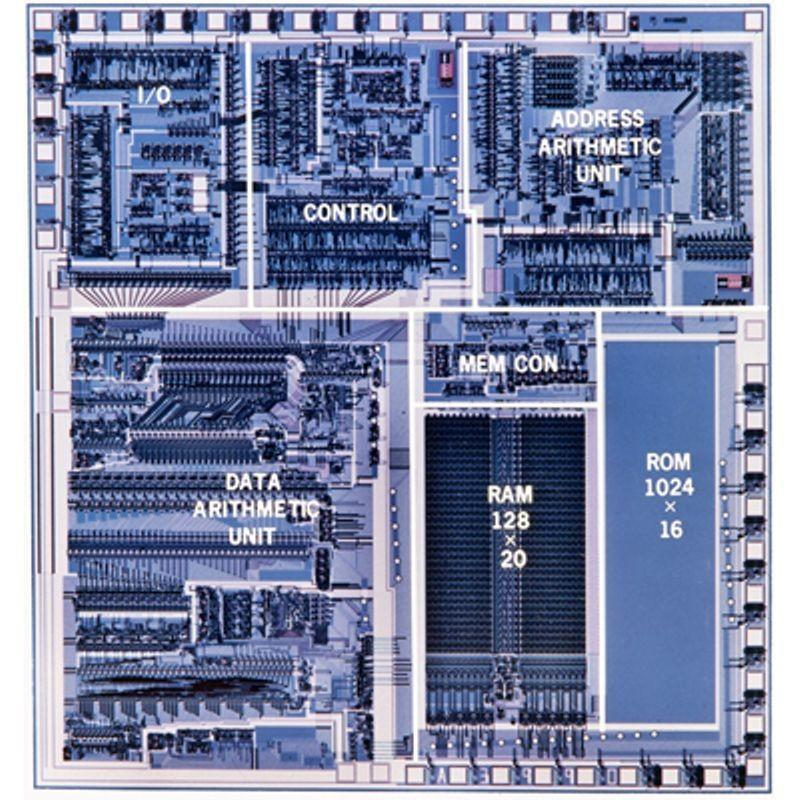
\includegraphics[width=\textwidth]{imgs/vis_5.jpg}
        \end{column}
        \begin{column}{0.5\textwidth}
            These elements usually make up your computer's central processing unit, or CPU.
            \vspace{\baselineskip}
            In reality, your computer can have more than one copy of a CPU "core" to do different things simultaneously, making it faster to compute overall.
            \vspace{\baselineskip}
            Your computer also has a bunch of extra hardware to handle power, graphics, storage, and interfacing with other things like your mouse, keyboard, screen, camera, USB port, wifi chip, ...
        \end{column}
    \end{columns}

\end{frame}

\begin{frame}{Making a Computer}
    
    \begin{columns}
        \begin{column}{0.5\textwidth}
            \begin{figure}
                \centering
                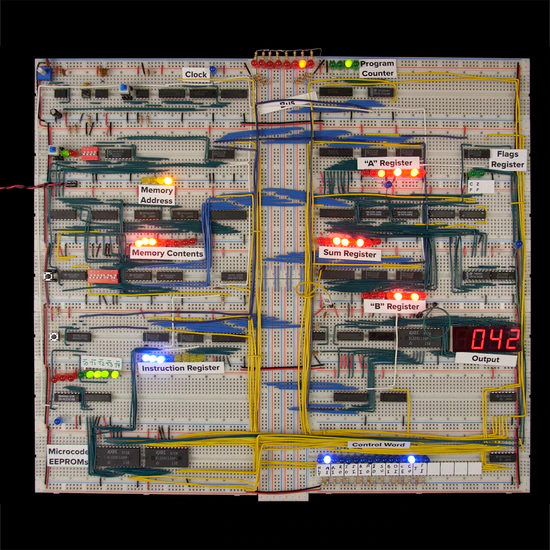
\includegraphics[width=0.9\textwidth]{imgs/vis_7.png}
                \\
                \href{https://eater.net/8bit}{"Build an 8-bit computer from scratch"}
            \end{figure}
        \end{column}
        \begin{column}{0.5\textwidth}
            You (yes you!) can make your own computer very easily from scratch. In fact RISC-V and other open-source hardware tools are commnly used by both students and professionals to do reseach and develop new hardware.
        \end{column}
    \end{columns}

\end{frame}

\begin{frame}{Making a Computer}

    \begin{columns}
        \begin{column}{0.5\textwidth}
            \begin{figure}
                \centering
                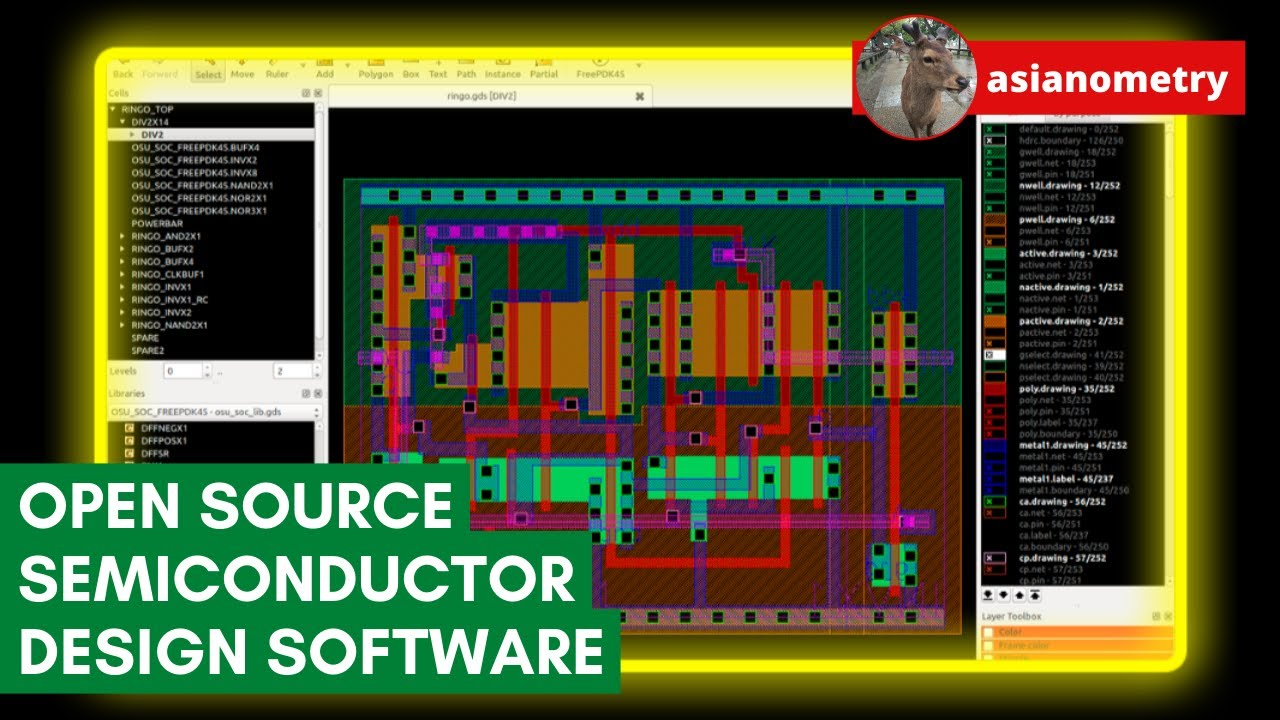
\includegraphics[width=\textwidth]{imgs/oseda.jpg}
                \\
                \href{https://www.youtube.com/watch?v=OmEbzRp_NGg}{"The Promise of Open Source Semiconductor Design Tools"}
            \end{figure}
        \end{column}
        \begin{column}{0.5\textwidth}
            \begin{figure}
                \centering
                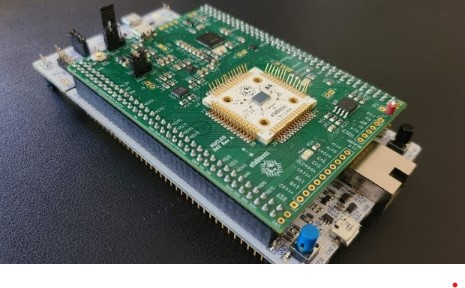
\includegraphics[width=\textwidth]{imgs/tapeout_chip.jpg}
                \\
                Example of a fabricated chip using open-source tools and fabrication technology
            \end{figure}
        \end{column}
    \end{columns}

\end{frame}

\section{Computer Software}

\begin{frame}{Computer Instructions}
    At the lowest level, each CPU hardware design has a set of basic instructions called an Instruction Set Architecture or \textbf{ISA}.
    
    \begin{itemize}
        \item Intel has an ISA called \texttt{x86}
        \item Many phones and Apple computers use an ISA called \texttt{ARM}
        \item Arduinos use an ISA called \texttt{AVR}
    \end{itemize}
    
    An ISA is an outline of the set of instructions that a CPU can perform.
    \begin{itemize}
        \item Add two numbers
        \item Move this number from location A to location B
        \item Compare two numbers or compare a number to zero
        \item Jump to this location in the code
        \item Run this block of code and come back when done
        \item Load and store this number in this location of memory
    \end{itemize}

\end{frame}

\begin{frame}{Computer Instructions}
    \begin{figure}
        \centering
        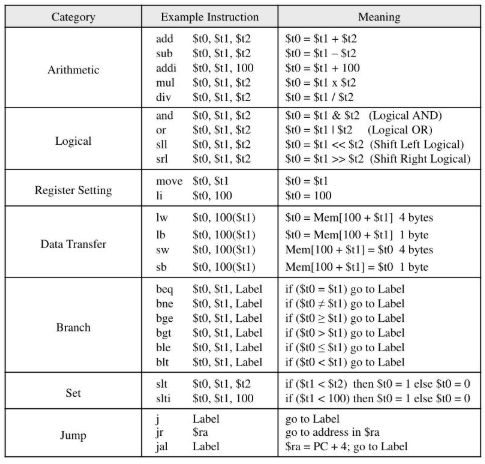
\includegraphics[width=0.5\textwidth]{imgs/vis_6.png}
        \\
        An example of a simple ISA
    \end{figure}
\end{frame}

\begin{frame}{Computer Instructions}
    \begin{figure}
        \centering
        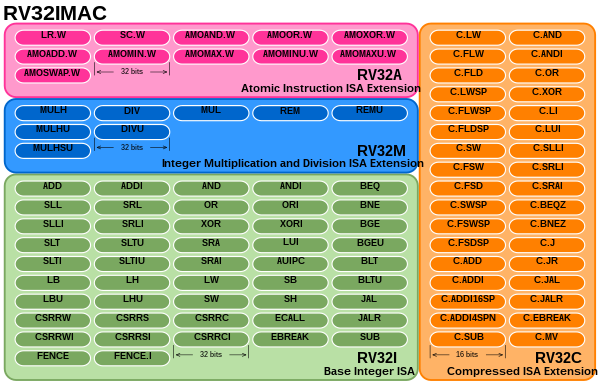
\includegraphics[width=0.6\textwidth]{imgs/RV32IMAC_Instruction_Set.svg.png}
        \\
        An example of a RISC-V ISA
    \end{figure}
\end{frame}

\begin{frame}{Programming Langauges}

    Programmers want a more expressive way to write programs for their computers with more features rather than just the assembly language

    \vspace{\baselineskip}

    They designed higher level languages that can be translated, aka compiled, into lower level code (ex. an ISA)

    \vspace{\baselineskip}

    These higher level languages have more useful features and better language and syntax
    % Standard libraries for things like math, file reading, networking, graphics, user interfaces 
    % Memory management
    % bullet points

    \begin{itemize}
        \item Standard libraries for things like math, file reading, networking, graphics, user interfaces
        \item Memory management
        \item Concurrency and parallelism
    \end{itemize}
    
\end{frame}

\begin{frame}{Programming Langauges}
    You can now build higher level functionality like a file system, a desktop user interface, user management, networking (wifi and ethernet), a way to run other applications, and a web browser

    \vspace{\baselineskip}
    
    All of a sudden you have an operating system
    \begin{itemize}
        \item That previous point kinda sounds like Chrome OS on your Chromebook
        \item Windows, Mac, Linux
    \end{itemize}

\end{frame}

\begin{frame}{Programming Langauges}

    \begin{figure}
        \centering
        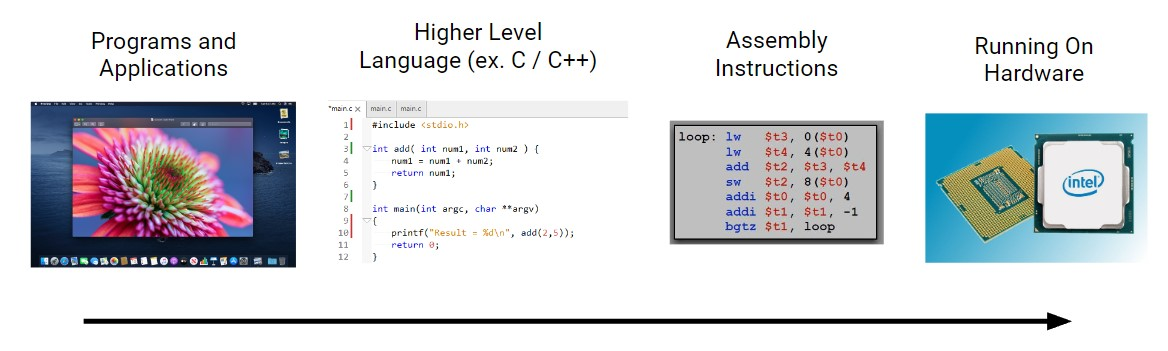
\includegraphics[width=\textwidth]{imgs/vis_8.jpg}
        \\
        Example of abstaction for software and hardware layers
    \end{figure}
\end{frame}

\end{document}